\documentclass[10pt]{beamer}

\usepackage[utf8]{inputenc}
\usepackage[french]{babel}

\usetheme[progressbar=frametitle]{metropolis}
\usepackage{appendixnumberbeamer}

\usepackage{booktabs}
\usepackage[scale=2]{ccicons}

\usepackage{pgfplots}
\usepgfplotslibrary{dateplot}

\usepackage{xspace}
\newcommand{\themename}{\textbf{\textsc{metropolis}}\xspace}

\usepackage{tikz}
\usepackage{svg}

\usepackage{amsthm}
\usepackage{amsfonts}
\usepackage{mathrsfs}

\usepackage{thmtools}

%\usetikzlibrary{graphs}
%\usetikzlibrary{graphs.standard}

\let\definition\relax
\let\theorem\relax
\newtheorem{definition}{Définition}[section]
\newtheorem{proposition}[definition]{Proposition}
\newtheorem{theorem}[definition]{Théorème}

\title{Polytopes abstraits réguliers de $A_{11}$}
%\subtitle{Graphes de Moore}
% \date{\today}
\date{}
\author{Nathan Meynaert}
% \titlegraphic{\hfill\includegraphics[height=1.5cm]{logo.pdf}}

\begin{document}

\maketitle

\begin{frame}{Objectifs}
  Dans l'étude des polytopes abstraits possédant un certain groupe d'automorphismes, le groupe $A_{11}$ est un peu spécial.

  Il a été calculé que ce groupe n'admet que des polytopes de rang 3 et de rang 6.

  C'est le seul exemple connu où l'ensemble des rangs admissibles n'est pas un intervalle.

  Il s'agit de comprendre pourquoi le groupe $A_{11}$ n'a pas de polytopes de rang 4 ou de rang 5 malgré le fait qu'il ait des polytopes de rang 3 et de rang 6.
\end{frame}

\begin{frame}{Table des matières}
  \setbeamertemplate{section in toc}[sections numbered]
  \tableofcontents[hideallsubsections]
\end{frame}

\section{Polytopes abstraits}

\begin{frame}{Définition}

  \begin{definition}
    Un \textit{polytope abstrait} est un ensemble partiellement ordonné, gradué,  dont les éléments sont appelés \textit{faces} et sont ordonnés par l'inclusion $\subseteq$ tels que
    \begin{itemize}
      \item \textbf{(P1)} $\mathcal P$ contient deux faces impropres: $F_{-1}$ et $F_d$.
      \item \textbf{(P2)} Les drapeaux de $\mathcal P$ contiennent $d+2$ faces (en incluant les deux faces impropres)    \item \textbf{(P3)} $\mathcal P$ est fortement connexe.
      \item \textbf{(P4)} $\mathcal P$ satisfait la propriété du diamant.
    \end{itemize}
  \end{definition}

\end{frame}

\begin{frame}{Fortement connexe}

  Un poset gradué est dit connexe, si son rang est $\le 1$ ou si, pour toute paire de points $x, y$ il existe une suite de points $x = x_0, \dots, x_n = y$ tels que $x_i$ et $x_{i+1}$ soient comparables.

  Une section $[x,z]$ d'un poset est l'ensemble des points $y$ du poset tels que  $x \le y \le z$.

  Un poset est fortement connexe si toute section du poset est connexe.

\end{frame}

\begin{frame}{Exemple (4)}
  \begin{figure}[H]
    \begin{center}
      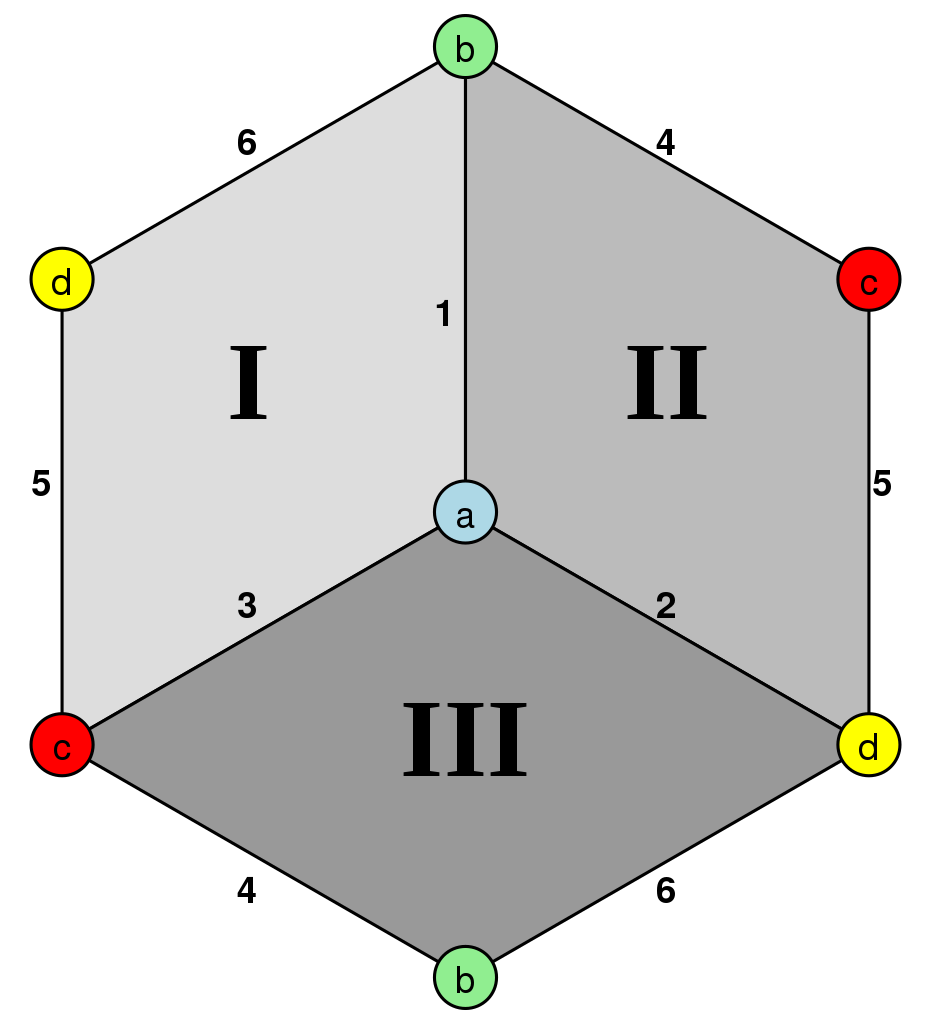
\includegraphics[width=7cm]{Hemicube.png}
    \end{center}
  \end{figure}
\end{frame}

\section{String C-group representations}

\begin{frame}{Définitions}
  \begin{definition}
    Un sggi est une suite de générateurs $\rho_0, \dots, \rho_{r-1}$ telle que les involutions non-consécutives commutent.
  \end{definition}


    Un sggi satisfait la propriété d'intersection si pour tout sous-ensemble $I, J$ de générateurs, on a
    \[
      \Gamma_{I} \cap \Gamma_{J} = \Gamma_{I \cap J}.
    \]

  \begin{definition}
    Un sggi qui satisfait la propriété d'intersection est appelé une string C-group representation.
  \end{definition}
\end{frame}

\begin{frame}{Dualité et propriétés}
  Il existe une correspondance entre les polytopes abstraits réguliers et les string C-groups representations.

  Pour y arriver, il faut prendre certains générateurs bien choisis du groupe d'automorphismes du polytope.

  Le dual d'un sggi est obtenu en inversant l'ordre des générateurs. Ceci donne aussi le dual du polytope.
\end{frame}

\begin{frame}{$i$-transpositions}
  Concentrons nous maintenant sur $A_{11}$.

  Les générateurs doivent être des involutions, dès lors ils doivent être des $i$-transpositions, c'est-à-dire que les générateurs permutent $i$ paires de points distincts.

  Le groupe $A_{11}$ ne contient que des permutations paires. Donc $i$ doit être pair mais ne peut pas être égal à 6 ou plus car il n'y a que 11 points.

  Les générateurs doivent donc être des 2-transpositions ou des 4-transpositions.
\end{frame}

\section{Permutation representation graphs}

\begin{frame}{Définition}
  Un permutation representation graph est un graphe représentant un sggi. Le sggi est composé de générateurs $\rho_0, \dots, \rho_{r-1}$. Ce graphe est un multigraphe avec labels dont les sommets sont les points du string C-group. Deux points $\alpha$ et $\beta$ sont reliés par une arête avec un label $i$ ssi $\alpha \rho_i = \beta$. Par convention, le graphe ne contient pas de boucle.


  \pause

  \begin{figure}[H]
    \begin{center}
      \begin{tikzpicture}[scale=.8]

        \begin{scope}[every node/.style={circle,draw, transform shape}]
          \node (1)  at (6,0)  {};
          \node (2)  at (6,2)  {};
          \node (3)  at (4,2)  {};
          \node (4)  at (4,0)  {};
          \node (5)  at (4,-2) {};
          \node (6)  at (2,-2) {};
          \node (7)  at (2,0)  {};
          \node (8)  at (2,2)  {};
          \node (9)  at (12,0) {};
          \node (10) at (10,0) {};
          \node (11) at (8,0) {};
        \end{scope}

        \begin{scope}[every node/.style={fill=white, transform shape}]

          \begin{scope}[every edge/.style={draw}]
            \path (1)  edge node {$0$} (2);
            \path (3)  edge node {$0$} (4);
            \path (5)  edge[bend right=50] node {$0$} (6);
            \path (7)  edge node {$0$} (8);
            \path (1)  edge node {$1$} (11);
            \path (3)  edge[bend right=30] node {$1$} (8);
            \path (4)  edge node {$1$} (5);
            \path (6)  edge node {$1$} (7);
            \path (1)  edge node {$2$} (4);
            \path (2)  edge node {$2$} (3);
            \path (5)  edge node {$2$} (6);
            \path (10) edge node {$2$} (11);
            \path (3)  edge[bend left=30] node {$3$} (8);
            \path (4)  edge node {$3$} (7);
            \path (5)  edge[bend left=50] node {$3$} (6);
            \path (9)  edge node {$3$} (10);
          \end{scope}
        \end{scope}

      \end{tikzpicture}
    \end{center}
  \end{figure}
\end{frame}

\begin{frame}{Motifs possibles}
  %Les générateurs non consecutifs d'un sggi doivent commuter, ceci a des conséquences sur le graphe.

  \begin{theorem}
    Dans un permutation representation graph, le graphe obtenu en ne conservant que les arêtes de deux générateurs non-consécutifs peut uniquement former les motifs suivants:
    \begin{itemize}
      \item Un point fixe
      \item Une arête simple
      \item Une arête double
      \item Un carré alterné
    \end{itemize}
  \end{theorem}

  \pause

  \begin{figure}[H]
    \begin{center}
      \begin{tikzpicture}[scale=.55]

        \begin{scope}[every node/.style={circle,draw, transform shape}]
          \node (1)  at (0,0)  {};
          \node (2)  at (2,0)  {};
          \node (3)  at (4,0)  {};
          \node (4)  at (6,0)  {};
          \node (5)  at (8,0) {};
          \node (6)  at (10,0) {};
          \node (7)  at (12,0)  {};
          \node (8)  at (14,0)  {};
          \node (9)  at (14,2) {};
          \node (10) at (16,0) {};
          \node (11) at (16,2) {};
        \end{scope}

        \begin{scope}[every node/.style={fill=white, transform shape}]

          \begin{scope}[every edge/.style={draw}]
            \path (2)  edge node {$i$} (3);
            \path (6)  edge[bend left=30] node {$i$} (7);
            \path (8)  edge node {$i$} (10);
            \path (9)  edge node {$i$} (11);
            \path (4)  edge node {$j$} (5);
            \path (6)  edge[bend right=30] node {$j$} (7);
            \path (8)  edge node {$j$} (9);
            \path (10) edge node {$j$} (11);
          \end{scope}
        \end{scope}

      \end{tikzpicture}
    \end{center}
  \end{figure}

\end{frame}

\begin{frame}{Exemple (1)}
  Un exemple:

  \begin{figure}[H]
    \begin{center}
      \begin{tikzpicture}[scale=.8]

        \begin{scope}[every node/.style={circle,draw, transform shape}]
          \node (1)  at (6,0)  {};
          \node (2)  at (6,2)  {};
          \node (3)  at (4,2)  {};
          \node (4)  at (4,0)  {};
          \node (5)  at (4,-2) {};
          \node (6)  at (2,-2) {};
          \node (7)  at (2,0)  {};
          \node (8)  at (2,2)  {};
          \node (9)  at (12,0) {};
          \node (10) at (10,0) {};
          \node (11) at (8,0) {};
        \end{scope}

        \begin{scope}[every node/.style={fill=white, transform shape}]

          \begin{scope}[every edge/.style={draw}]
            \path (1)  edge node {$0$} (2);
            \path (3)  edge node {$0$} (4);
            \path (5)  edge[bend right=50] node {$0$} (6);
            \path (7)  edge node {$0$} (8);
            \path (1)  edge node {$1$} (11);
            \path (3)  edge[bend right=30] node {$1$} (8);
            \path (4)  edge node {$1$} (5);
            \path (6)  edge node {$1$} (7);
            \path (1)  edge node {$2$} (4);
            \path (2)  edge node {$2$} (3);
            \path (5)  edge node {$2$} (6);
            \path (10) edge node {$2$} (11);
            \path (3)  edge[bend left=30] node {$3$} (8);
            \path (4)  edge node {$3$} (7);
            \path (5)  edge[bend left=50] node {$3$} (6);
            \path (9)  edge node {$3$} (10);
          \end{scope}
        \end{scope}

      \end{tikzpicture}
    \end{center}
  \end{figure}
\end{frame}

\begin{frame}{Exemple (2)}
  Un second exemple plus compliqué:

  \begin{figure}[H]
    \begin{center}
      \begin{tikzpicture}[scale=.8]

        \begin{scope}[every node/.style={circle,draw, transform shape}]
          \node (1)  at (0,2)  {h};
          \node (2)  at (0,0)  {g};
          \node (3)  at (0,-2) {f};
          \node (4)  at (-2,2)  {e};
          \node (5)  at (-2,0)  {d};
          \node (6)  at (-2,-2) {c};
          \node (7)  at (-4,2)  {b};
          \node (8)  at (-4,0)  {a};
          \node (9)  at (-2,4)  {i};
          \node (10) at (0,4)   {j};
          \node (11) at (2,0)   {k};
          \node (12) at (2,2)   {l};
        \end{scope}

        \begin{scope}[every node/.style={fill=white, transform shape}]

          \node (t1) at (-5,1)  {$i$};
          \node (t2) at (3,1)   {$i$};
          \node (t3) at (-1,-3) {$i+1$};
          \node (t4) at (-1,5)  {$i+1$};

          \begin{scope}[every edge/.style={draw}]
            \path (2)  edge node {$i+2$} (3);
            \path (5)  edge node {$i+2$} (6);
            \path (9)  edge node {$i+2$} (4);
            \path (10) edge node {$i+2$} (1);
            \path (1)  edge node {$i$} (2);
            \path (4)  edge node {$i$} (5);
            \path (7)  edge node {$i$} (8);
            \path (11) edge node {$i$} (12);
            \path (9)  edge[bend right=45] (t1);
            \path (t1) edge[bend right=45] (6);
            \path (10) edge[bend left=45] (t2);
            \path (t2) edge[bend left=45] (3);
            \path (12) edge[bend right=45] (t4);
            \path (t4) edge[bend right=45] (7);
            \path (11) edge[bend left=45] (t3);
            \path (t3) edge[bend left=45] (8);
            \path (1)  edge node {$i+1$} (4);
            \path (2)  edge node {$i+1$} (5);
            \path (3)  edge node {$i+1$} (6);
            \path (4)  edge node {$i+3$} (7);
            \path (5)  edge node {$i+3$} (8);
            \path (1)  edge node {$i+3$} (12);
            \path (2)  edge node {$i+3$} (11);
          \end{scope}
        \end{scope}

      \end{tikzpicture}
    \end{center}
  \end{figure}
\end{frame}

\section{En rang 5, il faut au moins une 4-transposition}

\begin{frame}{Objectif}
  \begin{theorem}
    Tout permutation representation graph de rang 5 de $A_{11}$ admet au moins une 4-transposition.
  \end{theorem}
\end{frame}

\begin{frame}{Preuve (1)}
    Supposons qu'il n'y ait aucune 4-transposition alors tous les générateurs doivent être des 2-transpositions. Donc il y a 10 arêtes pour lier 11 points. Le graphe doit donc être un arbre.

    Cependant aucun sommet ne peut être relié par 3 arêtes.

    \begin{figure}[H]
      \begin{center}
        \begin{tikzpicture}[scale=.8]

          \begin{scope}[every node/.style={circle,draw, transform shape}]
            \node (1)  at (0,0)  {};
            \node (2)  at (2,0)  {};
            \node (3)  at (4,0)  {};
            \node (4)  at (2,2)  {};
          \end{scope}

          \begin{scope}[every node/.style={fill=white, transform shape}]
            \begin{scope}[every edge/.style={draw}]
              \path (1)  edge node {$i$} (2);
              \path (2)  edge node {$j$} (3);
              \path (2)  edge node {$k$} (4);
            \end{scope}
          \end{scope}

        \end{tikzpicture}
      \end{center}
    \end{figure}

    Supposons que $i$ et $k$ soient non-consécutifs alors les deux arêtes $i$ et $k$ de ce graphe doivent être dans un motif valide. La seule possibilité est un carré alterné mais alors le graphe n'est pas un arbre.

    Donc le graphe doit être une chaîne.
\end{frame}

\begin{frame}{Preuve (2)}

  Dans une chaîne, les indices des arêtes adjacentes doivent être consécutifs. En particulier les arêtes $\rho_0$ ne peuvent être adjacentes qu'à des arêtes $\rho_1$.

  Vu qu'il y a deux arêtes de chaque type, une arête $\rho_0$ doit être à l'extrémité du graphe. Si une arête $\rho_0$ ne se trouve pas à l'extrémité du graphe, alors elle doit être entourée de deux arêtes $\rho_1$.

  \begin{figure}[H]
    \begin{center}
      \begin{tikzpicture}[scale=.8]

        \begin{scope}[every node/.style={circle,draw, transform shape}]
          \node (1)  at (0,0)  {};
          \node (2)  at (2,0)  {};
          \node (3)  at (4,0)  {};
          \node (4)  at (6,0)  {};
        \end{scope}

        \begin{scope}[every node/.style={fill=white, transform shape}]
          \begin{scope}[every edge/.style={draw}]
            \path (1)  edge node {$1$} (2);
            \path (2)  edge node {$0$} (3);
            \path (3)  edge node {$1$} (4);
          \end{scope}
        \end{scope}

      \end{tikzpicture}
    \end{center}
  \end{figure}

  \pause

  La seconde arête $\rho_0$ doit être adjacente à une de ces arêtes $\rho_1$ mais ne peut avoir d'arête adjacente à son autre extrémité.

  \begin{figure}[H]
    \begin{center}
      \begin{tikzpicture}[scale=.8]

        \begin{scope}[every node/.style={circle,draw, transform shape}]
          \node (0)  at (-2,0)  {};
          \node (1)  at (0,0)  {};
          \node (2)  at (2,0)  {};
          \node (3)  at (4,0)  {};
          \node (4)  at (6,0)  {};
        \end{scope}

        \begin{scope}[every node/.style={fill=white, transform shape}]
          \begin{scope}[every edge/.style={draw}]
            \path (0)  edge node {$0$} (1);
            \path (1)  edge node {$1$} (2);
            \path (2)  edge node {$0$} (3);
            \path (3)  edge node {$1$} (4);
          \end{scope}
        \end{scope}

      \end{tikzpicture}
    \end{center}
  \end{figure}



\end{frame}

\begin{frame}{Preuve (3)}
  Par dualité, la même conclusion s'applique à $\rho_4$, la chaîne doit donc commencer par ces motifs à chaque extrémité.

  \begin{figure}[H]
    \begin{center}
      \begin{tikzpicture}[scale=.5]

        \begin{scope}[every node/.style={circle,draw, transform shape}]
          \node (1)  at (0,0)  {};
          \node (2)  at (2,0)  {};
          \node (3)  at (4,0)  {};
          \node (4)  at (6,0)  {};
          \node (5)  at (8,0)  {};
          \node (7)  at (11,0) {};
          \node (8)  at (13,0) {};
          \node (9)  at (15,0) {};
          \node (10) at (17,0) {};
          \node (11) at (19,0) {};
        \end{scope}

        \node (5b) at (9,0) {};
        \node (7b) at (10,0) {};

        \begin{scope}[every node/.style={fill=white, transform shape}]

          \begin{scope}[every edge/.style={draw}]
            \path (1)  edge node {$0$} (2);
            \path (2)  edge node {$1$} (3);
            \path (3)  edge node {$0$} (4);
            \path (4)  edge node {$1$} (5);
            \path (5)  edge[style={dotted}] (5b);
            \path (7)  edge[style={dotted}] (7b);
            \path (7)  edge node {$3$} (8);
            \path (8)  edge node {$4$} (9);
            \path (9)  edge node {$3$} (10);
            \path (10) edge node {$4$} (11);
          \end{scope}
        \end{scope}
      \end{tikzpicture}
    \end{center}
  \end{figure}

  \pause

  Il ne reste que des arêtes $\rho_2$ à placer.

  \begin{figure}[H]
    \begin{center}
      \begin{tikzpicture}[scale=.5]

        \begin{scope}[every node/.style={circle,draw, transform shape}]
          \node (1)  at (0,0)  {};
          \node (2)  at (2,0)  {};
          \node (3)  at (4,0)  {};
          \node (4)  at (6,0)  {};
          \node (5)  at (8,0)  {};
          \node (6)  at (10,0)  {};
          \node (7)  at (12,0) {};
          \node (8)  at (14,0) {};
          \node (9)  at (16,0) {};
          \node (10) at (18,0) {};
          \node (11) at (20,0) {};
        \end{scope}

        \begin{scope}[every node/.style={fill=white, transform shape}]

          \begin{scope}[every edge/.style={draw}]
            \path (1)  edge node {$0$} (2);
            \path (2)  edge node {$1$} (3);
            \path (3)  edge node {$0$} (4);
            \path (4)  edge node {$1$} (5);
            \path (7)  edge node {$3$} (8);
            \path (8)  edge node {$4$} (9);
            \path (9)  edge node {$3$} (10);
            \path (10) edge node {$4$} (11);
          \end{scope}
        \end{scope}
      \end{tikzpicture}
    \end{center}
  \end{figure}

  Ce qui est clairement impossible et donc aucune chaîne ne peut être construite.

\end{frame}

\section{Méthode}

\begin{frame}{Méthode}
  Une méthode permettant de construire tous les graphes possibles est la suivante:

  \begin{enumerate}
    \item Partir d'une involution de base
    \item À partir d'une deuxième involution, sachant qu'il existe uniquement quatre motifs valides, lister toutes les possibilités.
    \item Étendre le graphe afin qu'il devienne connexe. Des arêtes supplémentaires peuvent être placées afin de satisfaire diverses contraintes.
    \item Ajouter les arêtes restantes.
  \end{enumerate}
\end{frame}

\section{Ni $\rho_0$ ni $\rho_4$ ne peut être une 4-transposition}

\begin{frame}{Intersection}
  Supposons que $\rho_0$ soit une 4-transposition, alors il permute 8 points. Cependant $\rho_4$ permute au moins 4 points et donc il existe un point qui est permuté par $\rho_0$ et $\rho_4$.

  Ce point doit faire partie d'un des 4 motifs. Les deux seuls possibles sont le carré alterné et l'arête double.

  Les motifs de départ sont donc les suivants:

  \begin{figure}[H]
    \begin{center}
      \begin{tikzpicture}[scale=.55]

        \begin{scope}[every node/.style={circle,draw, transform shape}]
          \node (6)  at (10,0) {};
          \node (7)  at (12,0) {};
          \node (8)  at (14,0) {};
          \node (9)  at (14,2) {};
          \node (10) at (16,0) {};
          \node (11) at (16,2) {};
        \end{scope}

        \begin{scope}[every node/.style={fill=white, transform shape}]

          \begin{scope}[every edge/.style={draw}]
            \path (6)  edge[bend left=30] node {$0$} (7);
            \path (8)  edge node {$0$} (10);
            \path (9)  edge node {$0$} (11);
            \path (6)  edge[bend right=30] node {$4$} (7);
            \path (8)  edge node {$4$} (9);
            \path (10) edge node {$4$} (11);
          \end{scope}
        \end{scope}

      \end{tikzpicture}
    \end{center}
  \end{figure}

\end{frame}

\begin{frame}{Carré alterné (1)}
  Dans le cas du carré alterné

  \begin{figure}[H]
    \begin{center}
      \begin{tikzpicture}[scale=.55]

        \begin{scope}[every node/.style={circle,draw, transform shape}]
          \node (1)  at (0,0) {};
          \node (2)  at (0,2) {};
          \node (3)  at (2,0) {};
          \node (4)  at (2,2) {};
        \end{scope}

        \begin{scope}[every node/.style={fill=white, transform shape}]

          \begin{scope}[every edge/.style={draw}]
            \path (1)  edge node {$0$} (3);
            \path (2)  edge node {$0$} (4);
            \path (1)  edge node {$4$} (2);
            \path (3)  edge node {$4$} (4);
          \end{scope}
        \end{scope}

      \end{tikzpicture}
    \end{center}
  \end{figure}

  \pause

  Ce carré alterné ne peut être adjacent à une arête qui n'est pas contenue dans un carré alterné.

  Il doit donc être adjacent à un autre carré alterné. Les possibilités sont un carré avec $\rho_0$ et $\rho_3$ ou un carré avec $\rho_1$ et $\rho_4$. Le second cas peut être ramené au premier par dualité.

  \pause

  \begin{figure}[H]
    \begin{center}
      \begin{tikzpicture}[scale=.55]

        \begin{scope}[every node/.style={circle,draw, transform shape}]
          \node (1)  at (0,0) {};
          \node (2)  at (0,2) {};
          \node (3)  at (2,0) {};
          \node (4)  at (2,2) {};
          \node (5)  at (4,0) {};
          \node (6)  at (4,2) {};
        \end{scope}

        \begin{scope}[every node/.style={fill=white, transform shape}]

          \begin{scope}[every edge/.style={draw}]
            \path (1)  edge node {$0$} (2);
            \path (3)  edge node {$0$} (4);
            \path (5)  edge node {$0$} (6);
            \path (5)  edge node {$3$} (3);
            \path (6)  edge node {$3$} (4);
            \path (1)  edge node {$4$} (3);
            \path (2)  edge node {$4$} (4);
          \end{scope}
        \end{scope}

      \end{tikzpicture}
    \end{center}
  \end{figure}

\end{frame}

\begin{frame}{Carré alterné (2)}
  \begin{figure}[H]
    \begin{center}
      \begin{tikzpicture}[scale=.55]

        \begin{scope}[every node/.style={circle,draw, transform shape}]
          \node (1)  at (0,0) {};
          \node (2)  at (0,2) {};
          \node (3)  at (2,0) {};
          \node (4)  at (2,2) {};
          \node (5)  at (4,0) {};
          \node (6)  at (4,2) {};
        \end{scope}

        \begin{scope}[every node/.style={fill=white, transform shape}]

          \begin{scope}[every edge/.style={draw}]
            \path (1)  edge node {$0$} (2);
            \path (3)  edge node {$0$} (4);
            \path (5)  edge node {$0$} (6);
            \path (5)  edge node {$3$} (3);
            \path (6)  edge node {$3$} (4);
            \path (1)  edge node {$4$} (3);
            \path (2)  edge node {$4$} (4);
          \end{scope}
        \end{scope}

      \end{tikzpicture}
    \end{center}
  \end{figure}

  Un troisième carré alterné doit être placé, ce carré doit être composé de $\rho_0$ et $\rho_2$.

  \pause

  \begin{figure}[H]
    \begin{center}
      \begin{tikzpicture}[scale=.55]

        \begin{scope}[every node/.style={circle,draw, transform shape}]
          \node (1)  at (0,0) {};
          \node (2)  at (0,2) {};
          \node (3)  at (2,0) {};
          \node (4)  at (2,2) {};
          \node (5)  at (4,0) {};
          \node (6)  at (4,2) {};
          \node (7)  at (6,0) {};
          \node (8)  at (6,2) {};
        \end{scope}

        \begin{scope}[every node/.style={fill=white, transform shape}]

          \begin{scope}[every edge/.style={draw}]
            \path (1)  edge node {$0$} (2);
            \path (3)  edge node {$0$} (4);
            \path (5)  edge node {$0$} (6);
            \path (7)  edge node {$0$} (8);
            \path (5)  edge node {$2$} (7);
            \path (6)  edge node {$2$} (8);
            \path (5)  edge node {$3$} (3);
            \path (6)  edge node {$3$} (4);
            \path (1)  edge node {$4$} (3);
            \path (2)  edge node {$4$} (4);
          \end{scope}
        \end{scope}

      \end{tikzpicture}
    \end{center}
  \end{figure}

\end{frame}

\begin{frame}{Carré alterné (3)}
  \begin{figure}[H]
    \begin{center}
      \begin{tikzpicture}[scale=.55]

        \begin{scope}[every node/.style={circle,draw, transform shape}]
          \node (1)  at (0,0) {};
          \node (2)  at (0,2) {};
          \node (3)  at (2,0) {};
          \node (4)  at (2,2) {};
          \node (5)  at (4,0) {};
          \node (6)  at (4,2) {};
          \node (7)  at (6,0) {};
          \node (8)  at (6,2) {};
        \end{scope}

        \begin{scope}[every node/.style={fill=white, transform shape}]

          \begin{scope}[every edge/.style={draw}]
            \path (1)  edge node {$0$} (2);
            \path (3)  edge node {$0$} (4);
            \path (5)  edge node {$0$} (6);
            \path (7)  edge node {$0$} (8);
            \path (5)  edge node {$2$} (7);
            \path (6)  edge node {$2$} (8);
            \path (5)  edge node {$3$} (3);
            \path (6)  edge node {$3$} (4);
            \path (1)  edge node {$4$} (3);
            \path (2)  edge node {$4$} (4);
          \end{scope}
        \end{scope}

      \end{tikzpicture}
    \end{center}
  \end{figure}

  Maintenant il est possible de connecter une arête simple, celle-ci doit être $\rho_1$.

  \pause

  \begin{figure}[H]
    \begin{center}
      \begin{tikzpicture}[scale=.55]

        \begin{scope}[every node/.style={circle,draw, transform shape}]
          \node (1)  at (0,0) {};
          \node (2)  at (0,2) {};
          \node (3)  at (2,0) {};
          \node (4)  at (2,2) {};
          \node (5)  at (4,0) {};
          \node (6)  at (4,2) {};
          \node (7)  at (6,0) {};
          \node (8)  at (6,2) {};
          \node (9)  at (8,0) {};
        \end{scope}

        \begin{scope}[every node/.style={fill=white, transform shape}]

          \begin{scope}[every edge/.style={draw}]
            \path (1)  edge node {$0$} (2);
            \path (3)  edge node {$0$} (4);
            \path (5)  edge node {$0$} (6);
            \path (7)  edge node {$0$} (8);
            \path (7)  edge node {$1$} (9);
            \path (5)  edge node {$2$} (7);
            \path (6)  edge node {$2$} (8);
            \path (5)  edge node {$3$} (3);
            \path (6)  edge node {$3$} (4);
            \path (1)  edge node {$4$} (3);
            \path (2)  edge node {$4$} (4);
          \end{scope}
        \end{scope}

      \end{tikzpicture}
    \end{center}
  \end{figure}

  Maintenant une arête $\rho_2$ doit être placée.

  \begin{figure}[H]
    \begin{center}
      \begin{tikzpicture}[scale=.55]

        \begin{scope}[every node/.style={circle,draw, transform shape}]
          \node (1)  at (0,0) {};
          \node (2)  at (0,2) {};
          \node (3)  at (2,0) {};
          \node (4)  at (2,2) {};
          \node (5)  at (4,0) {};
          \node (6)  at (4,2) {};
          \node (7)  at (6,0) {};
          \node (8)  at (6,2) {};
          \node (9)  at (8,0) {};
          \node (10) at (10,0) {};
        \end{scope}

        \begin{scope}[every node/.style={fill=white, transform shape}]

          \begin{scope}[every edge/.style={draw}]
            \path (1)  edge node {$0$} (2);
            \path (3)  edge node {$0$} (4);
            \path (5)  edge node {$0$} (6);
            \path (7)  edge node {$0$} (8);
            \path (7)  edge node {$1$} (9);
            \path (5)  edge node {$2$} (7);
            \path (6)  edge node {$2$} (8);
            \path (9)  edge node {$2$} (10);
            \path (5)  edge node {$3$} (3);
            \path (6)  edge node {$3$} (4);
            \path (1)  edge node {$4$} (3);
            \path (2)  edge node {$4$} (4);
          \end{scope}
        \end{scope}

      \end{tikzpicture}
    \end{center}
  \end{figure}
\end{frame}

\begin{frame}{Carré alterné (4)}
  \begin{figure}[H]
    \begin{center}
      \begin{tikzpicture}[scale=.55]

        \begin{scope}[every node/.style={circle,draw, transform shape}]
          \node (1)  at (0,0) {};
          \node (2)  at (0,2) {};
          \node (3)  at (2,0) {};
          \node (4)  at (2,2) {};
          \node (5)  at (4,0) {};
          \node (6)  at (4,2) {};
          \node (7)  at (6,0) {};
          \node (8)  at (6,2) {};
          \node (9)  at (8,0) {};
          \node (10) at (10,0) {};
        \end{scope}

        \begin{scope}[every node/.style={fill=white, transform shape}]

          \begin{scope}[every edge/.style={draw}]
            \path (1)  edge node {$0$} (2);
            \path (3)  edge node {$0$} (4);
            \path (5)  edge node {$0$} (6);
            \path (7)  edge node {$0$} (8);
            \path (7)  edge node {$1$} (9);
            \path (5)  edge node {$2$} (7);
            \path (6)  edge node {$2$} (8);
            \path (9)  edge node {$2$} (10);
            \path (5)  edge node {$3$} (3);
            \path (6)  edge node {$3$} (4);
            \path (1)  edge node {$4$} (3);
            \path (2)  edge node {$4$} (4);
          \end{scope}
        \end{scope}

      \end{tikzpicture}
    \end{center}
  \end{figure}

  Un point doit encore être relié mais le nombre total d'arêtes $\rho_2$ est pour le moment impair.

  La dernière arête $\rho_2$ doit donc soit lier le dernier point à cette composante, soit lier deux points dejà dans cette même composante.

  Aucune de ces options n'est possible donc aucun permutation representation graph ne peut être trouvé.


\end{frame}

\section{Ni $\rho_1$ ni $\rho_3$ ne peut être une 4-transposition}

\begin{frame}{Graphes possibles}

  Après application de la méthode dans ce cas, nous trouvons deux familles de graphes. Voici un exemple pour chaque famille.

  \begin{figure}[H]
    \begin{center}
      \begin{tikzpicture}[scale=.55]

        \begin{scope}[every node/.style={circle,draw, transform shape}]
          \node (1)  at (0,2)  {};
          \node (2)  at (0,0)  {};
          \node (3)  at (2,2)  {};
          \node (4)  at (2,0)  {};
          \node (5)  at (4,2)  {};
          \node (6)  at (4,0)  {};
          \node (7)  at (6,0)  {};
          \node (8)  at (8,2)  {};
          \node (9)  at (8,0)  {};
          \node (10) at (10,2) {};
          \node (11) at (10,0) {};
        \end{scope}

        \begin{scope}[every node/.style={fill=white, transform shape}]

          \begin{scope}[every edge/.style={draw}]
            \path (9)  edge node {$0$} (11);
            \path (8)  edge[bend left=30] node {$0$} (10);
            \path (1)  edge[bend right=30] node {$1$} (2);
            \path (3)  edge node {$1$} (4);
            \path (5)  edge node {$1$} (6);
            \path (7)  edge node {$1$} (9);
            \path (1)  edge[bend left=30] node {$2$} (3);
            \path (6)  edge node {$2$} (7);
            \path (8)  edge node {$2$} (9);
            \path (10) edge node {$2$} (11);
            \path (1)  edge[bend left=30] node {$3$} (2);
            \path (3)  edge node {$3$} (5);
            \path (4)  edge node {$3$} (6);
            \path (8)  edge[bend right=30] node {$3$} (10);
            \path (1)  edge[bend right=30] node {$4$} (3);
            \path (2)  edge node {$4$} (4);
          \end{scope}
        \end{scope}

      \end{tikzpicture}
    \end{center}
  \end{figure}

  \begin{figure}[H]
    \begin{center}
      \begin{tikzpicture}[scale=.55]

        \begin{scope}[every node/.style={circle,draw, transform shape}]
          \node (1)  at (0,2)  {};
          \node (2)  at (0,0)  {};
          \node (3)  at (2,2)  {};
          \node (4)  at (2,0)  {};
          \node (5)  at (4,0)  {};
          \node (6)  at (6,0)  {};
          \node (7)  at (8,0)  {};
          \node (8)  at (10,0) {};
          \node (9)  at (-2,2) {};
          \node (10) at (-2,0) {};
          \node (11) at (12,0) {};
        \end{scope}

        \begin{scope}[every node/.style={fill=white, transform shape}]

          \begin{scope}[every edge/.style={draw}]
            \path (6)  edge[bend left=30] node {$0$} (7);
            \path (8)  edge node {$0$} (11);
            \path (1)  edge[bend right=30] node {$1$} (2);
            \path (3)  edge node {$1$} (4);
            \path (5)  edge node {$1$} (6);
            \path (7)  edge node {$1$} (8);
            \path (1)  edge node {$2$} (9);
            \path (2)  edge node {$2$} (10);
            \path (4)  edge node {$2$} (5);
            \path (6)  edge[bend right=30] node {$2$} (7);
            \path (1)  edge node {$3$} (3);
            \path (2)  edge node {$3$} (4);
            \path (1)  edge[bend left=30] node {$4$} (2);
            \path (9)  edge node {$4$} (10);
          \end{scope}
        \end{scope}

      \end{tikzpicture}
    \end{center}
  \end{figure}

  Nous allons maintenant essayer de prouver que les générateurs de ces graphes ne sont pas indépendants.

\end{frame}

\begin{frame}{Premier graphe}

  Reprenons le premier graphe.

  \begin{figure}[H]
    \begin{center}
      \begin{tikzpicture}[scale=.55]

        \begin{scope}[every node/.style={circle,draw, transform shape}]
          \node (1)  at (0,2)  {};
          \node (2)  at (0,0)  {};
          \node (3)  at (2,2)  {};
          \node (4)  at (2,0)  {};
          \node (5)  at (4,2)  {};
          \node (6)  at (4,0)  {};
          \node (7)  at (6,0)  {};
          \node (8)  at (8,2)  {};
          \node (9)  at (8,0)  {};
          \node (10) at (10,2) {};
          \node (11) at (10,0) {};
        \end{scope}

        \begin{scope}[every node/.style={fill=white, transform shape}]

          \begin{scope}[every edge/.style={draw}]
            \path (9)  edge node {$0$} (11);
            \path (8)  edge[bend left=30] node {$0$} (10);
            \path (1)  edge[bend right=30] node {$1$} (2);
            \path (3)  edge node {$1$} (4);
            \path (5)  edge node {$1$} (6);
            \path (7)  edge node {$1$} (9);
            \path (1)  edge[bend left=30] node {$2$} (3);
            \path (6)  edge node {$2$} (7);
            \path (8)  edge node {$2$} (9);
            \path (10) edge node {$2$} (11);
            \path (1)  edge[bend left=30] node {$3$} (2);
            \path (3)  edge node {$3$} (5);
            \path (4)  edge node {$3$} (6);
            \path (8)  edge[bend right=30] node {$3$} (10);
            \path (1)  edge[bend right=30] node {$4$} (3);
            \path (2)  edge node {$4$} (4);
          \end{scope}
        \end{scope}

      \end{tikzpicture}
    \end{center}
  \end{figure}

  Conservons uniquement les arêtes $\rho_1$, $\rho_2$ et $\rho_4$.

  \begin{figure}[H]
    \begin{center}
      \begin{tikzpicture}[scale=.55]

        \begin{scope}[every node/.style={circle,draw, transform shape}]
          \node (1)  at (0,2)  {};
          \node (2)  at (0,0)  {};
          \node (3)  at (2,2)  {};
          \node (4)  at (2,0)  {};
          \node (5)  at (6,0)  {};
          \node (6)  at (4,0)  {};
          \node (7)  at (8,0)  {};
          \node (8)  at (10,0)  {};
          \node (9)  at (12,0)  {};
          \node (10) at (14,0)  {};
          \node (11) at (16,0) {};
        \end{scope}

        \begin{scope}[every node/.style={fill=white, transform shape}]

          \begin{scope}[every edge/.style={draw}]
            \path (1)  edge node {$1$} (2);
            \path (3)  edge node {$1$} (4);
            \path (5)  edge node {$1$} (6);
            \path (7)  edge node {$1$} (8);
            \path (1)  edge[bend left=30] node {$2$} (3);
            \path (5)  edge node {$2$} (7);
            \path (8)  edge node {$2$} (9);
            \path (10) edge node {$2$} (11);
            \path (1)  edge[bend right=30] node {$4$} (3);
            \path (2)  edge node {$4$} (4);
          \end{scope}
        \end{scope}

      \end{tikzpicture}
    \end{center}
  \end{figure}

  \pause

  Il apparaît clairement que $\rho_4 = (\rho_1 \rho_2)^{10}$.

  Donc la propriété d'intersection ne peut être vérifiée.

\end{frame}

\begin{frame}{Second graphe (1)}

  Dans le cas du second graphe.

  \begin{figure}[H]
    \begin{center}
      \begin{tikzpicture}[scale=.55]

        \begin{scope}[every node/.style={circle,draw, transform shape}]
          \node (1)  at (0,2)  {};
          \node (2)  at (0,0)  {};
          \node (3)  at (2,2)  {};
          \node (4)  at (2,0)  {};
          \node (5)  at (4,0)  {};
          \node (6)  at (6,0)  {};
          \node (7)  at (8,0)  {};
          \node (8)  at (10,0) {};
          \node (9)  at (-2,2) {};
          \node (10) at (-2,0) {};
          \node (11) at (12,0) {};
        \end{scope}

        \begin{scope}[every node/.style={fill=white, transform shape}]

          \begin{scope}[every edge/.style={draw}]
            \path (6)  edge[bend left=30] node {$0$} (7);
            \path (8)  edge node {$0$} (11);
            \path (1)  edge[bend right=30] node {$1$} (2);
            \path (3)  edge node {$1$} (4);
            \path (5)  edge node {$1$} (6);
            \path (7)  edge node {$1$} (8);
            \path (1)  edge node {$2$} (9);
            \path (2)  edge node {$2$} (10);
            \path (4)  edge node {$2$} (5);
            \path (6)  edge[bend right=30] node {$2$} (7);
            \path (1)  edge node {$3$} (3);
            \path (2)  edge node {$3$} (4);
            \path (1)  edge[bend left=30] node {$4$} (2);
            \path (9)  edge node {$4$} (10);
          \end{scope}
        \end{scope}

      \end{tikzpicture}
    \end{center}
  \end{figure}

  Retirons les arêtes $\rho_4$.

  \begin{figure}[H]
    \begin{center}
      \begin{tikzpicture}[scale=.55]

        \begin{scope}[every node/.style={circle,draw, transform shape}]
          \node (1)  at (0,2)  {};
          \node (2)  at (0,0)  {};
          \node (3)  at (2,2)  {};
          \node (4)  at (2,0)  {};
          \node (5)  at (4,0)  {};
          \node (6)  at (6,0)  {};
          \node (7)  at (8,0)  {};
          \node (8)  at (10,0) {};
          \node (9)  at (-2,2) {};
          \node (10) at (-2,0) {};
          \node (11) at (12,0) {};
        \end{scope}

        \begin{scope}[every node/.style={fill=white, transform shape}]

          \begin{scope}[every edge/.style={draw}]
            \path (6)  edge[bend left=30] node {$0$} (7);
            \path (8)  edge node {$0$} (11);
            \path (1)  edge node {$1$} (2);
            \path (3)  edge node {$1$} (4);
            \path (5)  edge node {$1$} (6);
            \path (7)  edge node {$1$} (8);
            \path (1)  edge node {$2$} (9);
            \path (2)  edge node {$2$} (10);
            \path (4)  edge node {$2$} (5);
            \path (6)  edge[bend right=30] node {$2$} (7);
            \path (1)  edge node {$3$} (3);
            \path (2)  edge node {$3$} (4);
          \end{scope}
        \end{scope}

      \end{tikzpicture}
    \end{center}
  \end{figure}

  Nous allons prouver que ce graphe génère $A_{11}$ et donc que $\rho_4$ peut être exprimé comme un produit des autres générateurs.

\end{frame}

\begin{frame}{Second graphe (2)}
  \begin{figure}[H]
    \begin{center}
      \begin{tikzpicture}[scale=.55]

        \begin{scope}[every node/.style={circle,draw, transform shape}]
          \node (1)  at (0,2)  {};
          \node (2)  at (0,0)  {};
          \node (3)  at (2,2)  {};
          \node (4)  at (2,0)  {};
          \node (5)  at (4,0)  {};
          \node (6)  at (6,0)  {};
          \node (7)  at (8,0)  {};
          \node (8)  at (10,0) {};
          \node (9)  at (-2,2) {};
          \node (10) at (-2,0) {};
          \node (11) at (12,0) {};
        \end{scope}

        \begin{scope}[every node/.style={fill=white, transform shape}]

          \begin{scope}[every edge/.style={draw}]
            \path (6)  edge[bend left=30] node {$0$} (7);
            \path (8)  edge node {$0$} (11);
            \path (1)  edge node {$1$} (2);
            \path (3)  edge node {$1$} (4);
            \path (5)  edge node {$1$} (6);
            \path (7)  edge node {$1$} (8);
            \path (1)  edge node {$2$} (9);
            \path (2)  edge node {$2$} (10);
            \path (4)  edge node {$2$} (5);
            \path (6)  edge[bend right=30] node {$2$} (7);
            \path (1)  edge node {$3$} (3);
            \path (2)  edge node {$3$} (4);
          \end{scope}
        \end{scope}

      \end{tikzpicture}
    \end{center}
  \end{figure}

  Ce graphe est 2-transitif, il est donc primitif. Dès lors il est possible d'utiliser la classification des groupes primitifs afin de prouver que ce graphe génère $A_{11}$. Le sous-groupe généré par $\rho_2$ et $\rho_3$ est $D_{24}$, l'ordre du groupe doit donc être un multiple de 1320.

  Il y a trois possibilités pour un tel ordre: $M_{11}$, $A_{11}$ ou $S_{11}$. La première est impossible car $M_{11}$ n'a pas $D_{24}$ comme sous-groupe et $S_{11}$ est impossible car tous les générateurs sont des permutations paires. Ce graphe doit donc générer $A_{11}$.

\end{frame}

\section{$\rho_2$ ne peut être une 4-transposition}

\begin{frame}{Résultats}
  Après avoir généré tous les graphes de permutations et éliminé ceux dont les générateurs ne sont pas indépendants, on trouve 6 graphes. En voici un exemple:

  \begin{figure}[H]
    \begin{center}
      \begin{tikzpicture}[scale=.55]

        \begin{scope}[every node/.style={circle,draw, transform shape}]
          \node (1)  at (0,0)  {};
          \node (2)  at (2,0)  {};
          \node (3)  at (4,0)  {};
          \node (4)  at (6,0)  {};
          \node (5)  at (8,0)  {};
          \node (6)  at (10,0)  {};
          \node (7)  at (14,2)  {};
          \node (8)  at (12,2)  {};
          \node (9)  at (12,0)  {};
          \node (10) at (14,0)  {};
          \node (11) at (16,0) {};
        \end{scope}

        \begin{scope}[every node/.style={fill=white, transform shape}]

          \begin{scope}[every edge/.style={draw}]
            \path (1)  edge node {$0$} (2);
            \path (3)  edge[bend left=30] node {$0$} (4);
            \path (2)  edge node {$1$} (3);
            \path (4)  edge node {$1$} (5);
            \path (3)  edge[bend right=30] node {$2$} (4);
            \path (5)  edge node {$2$} (6);
            \path (7)  edge node {$2$} (8);
            \path (9)  edge node {$2$} (10);
            \path (6)  edge node {$3$} (9);
            \path (10) edge node {$3$} (11);
            \path (7)  edge node {$4$} (10);
            \path (8)  edge node {$4$} (9);
          \end{scope}
        \end{scope}

      \end{tikzpicture}
    \end{center}
  \end{figure}

  \pause

  Prouvons que ce graphe n'est pas une string C-group representation car il ne satisfait pas la propriété d'intersection. Avec $I = \{\rho_1,\rho_2\}$ et $J = \{\rho_2,\rho_3,\rho_4\}$, nous prouvons que $\Gamma_I \cap \Gamma_J \neq \Gamma_{I \cap J} = \Gamma_{\rho_2}$.


\end{frame}

\begin{frame}{$I$}
  Pour $I = \{\rho_1,\rho_2\}$, le graphe est le suivant

  \begin{figure}[H]
    \begin{center}
      \begin{tikzpicture}[scale=.55]

        \begin{scope}[every node/.style={circle,draw, transform shape}]
          \node (1)  at (0,0)  {};
          \node (2)  at (2,0)  {};
          \node (3)  at (4,0)  {a};
          \node (4)  at (6,0)  {b};
          \node (5)  at (8,0)  {c};
          \node (6)  at (10,0)  {d};
          \node (7)  at (14,2)  {};
          \node (8)  at (12,2)  {};
          \node (9)  at (12,0)  {};
          \node (10) at (14,0)  {};
          \node (11) at (16,0) {};
        \end{scope}

        \begin{scope}[every node/.style={fill=white, transform shape}]

          \begin{scope}[every edge/.style={draw}]
            \path (2)  edge node {$1$} (3);
            \path (4)  edge node {$1$} (5);
            \path (3)  edge node {$2$} (4);
            \path (5)  edge node {$2$} (6);
            \path (7)  edge node {$2$} (8);
            \path (9)  edge node {$2$} (10);
          \end{scope}
        \end{scope}

      \end{tikzpicture}
    \end{center}
  \end{figure}

  \pause

  Puisque $(\rho_1\rho_2)^4 \rho_1 = (a~b)(c~d)$, il est possible de permuter quatre points reliés par des arêtes $\rho_2$ sans permuter les 4 autres. Cette permutation n'est clairement pas dans $\Gamma_{\rho_2}$.
\end{frame}

\begin{frame}{$J$ (1)}
  Pour $J = \{\rho_2, \rho_3, \rho_4\}$.

  \begin{figure}[H]
    \begin{center}
      \begin{tikzpicture}[scale=.55]

        \begin{scope}[every node/.style={circle,draw, transform shape}]
          \node (1)  at (0,0)  {};
          \node (2)  at (2,0)  {};
          \node (3)  at (4,0)  {};
          \node (4)  at (6,0)  {};
          \node (5)  at (8,0)  {};
          \node (6)  at (10,0)  {};
          \node (7)  at (14,2)  {};
          \node (8)  at (12,2)  {};
          \node (9)  at (12,0)  {};
          \node (10) at (14,0)  {};
          \node (11) at (16,0) {};
        \end{scope}

        \begin{scope}[every node/.style={fill=white, transform shape}]

          \begin{scope}[every edge/.style={draw}]
            \path (3)  edge node {$2$} (4);
            \path (5)  edge node {$2$} (6);
            \path (7)  edge node {$2$} (8);
            \path (9)  edge node {$2$} (10);
            \path (6)  edge node {$3$} (9);
            \path (10) edge node {$3$} (11);
            \path (7)  edge node {$4$} (10);
            \path (8)  edge node {$4$} (9);
          \end{scope}
        \end{scope}

      \end{tikzpicture}
    \end{center}
  \end{figure}

  \pause

  Le groupe généré par la composante de droite sur 7 points est $S_7$.

  En effet, le groupe est 2-transitif et donc primitif. Le sous-groupe généré par $\rho_2$ et $\rho_3$ est d'ordre 10. Donc l'ordre du groupe doit être un multiple de 210.

  \pause

  Les seules possibilités sont $A_7$ et $S_7$. Vu que $\rho_2$ est une permutation impaire dans ce groupe, ce ne peut être que $S_7$.
\end{frame}

\begin{frame}{$J$ (2)}
  \begin{figure}[H]
    \begin{center}
      \begin{tikzpicture}[scale=.55]

        \begin{scope}[every node/.style={circle,draw, transform shape}]
          \node (1)  at (0,0)  {};
          \node (2)  at (2,0)  {};
          \node (3)  at (4,0)  {};
          \node (4)  at (6,0)  {};
          \node (5)  at (8,0)  {};
          \node (6)  at (10,0)  {};
          \node (7)  at (14,2)  {};
          \node (8)  at (12,2)  {};
          \node (9)  at (12,0)  {};
          \node (10) at (14,0)  {};
          \node (11) at (16,0) {};
        \end{scope}

        \begin{scope}[every node/.style={fill=white, transform shape}]

          \begin{scope}[every edge/.style={draw}]
            \path (3)  edge node {$2$} (4);
            \path (5)  edge node {$2$} (6);
            \path (7)  edge node {$2$} (8);
            \path (9)  edge node {$2$} (10);
            \path (6)  edge node {$3$} (9);
            \path (10) edge node {$3$} (11);
            \path (7)  edge node {$4$} (10);
            \path (8)  edge node {$4$} (9);
          \end{scope}
        \end{scope}

      \end{tikzpicture}
    \end{center}
  \end{figure}


  Vu que le groupe est $S_7$ l'arête isolée permet que la permutation prise sur le graphe dans son ensemble soit paire. Toutes les permutations de 4 points de $\rho_2$ se trouvent dans le groupe représenté par ce graphe. En particulier la permutation que nous avons trouvée pour $\Gamma_I$ s'y trouve.

  Donc il existe une permutation qui est dans $\Gamma_I$ et dans $\Gamma_J$ mais pas dans $\Gamma_{I \cap J}$. Ce sggi n'est donc pas une string C-group representation.

\end{frame}

\section{Conclusion}

\begin{frame}{Et le rang 6?}
  Pourquoi est-ce qu'il existe de polytopes de rang 6 alors?

  \pause

  En rang 6, il est possible de n'avoir que des 2-transpositions. Dans ce cas, on a quand même 12 arêtes pour lier 11 points.

  La différence est que l'on est plus capable de construire des motifs d'intersection entre les involutions non-consécutives car on est plus sûr qu'elle partagent effectivement un sommet.

  Ceci retire des contraintes et permet quand même de former 3 polytopes.
\end{frame}

\begin{frame}{Polytopes de rang 6}

  \begin{figure}[H]
    \begin{center}
      \begin{tikzpicture}[scale=.55]

        \begin{scope}[every node/.style={circle,draw, transform shape}]
          \node (1)  at (0,0)  {};
          \node (2)  at (2,0)  {};
          \node (3)  at (4,0)  {};
          \node (4)  at (6,0)  {};
          \node (5)  at (8,0)  {};
          \node (6)  at (10,0)  {};
          \node (7)  at (12,0)  {};
          \node (8)  at (14,0)  {};
          \node (9)  at (16,0)  {};
          \node (10) at (18,0)  {};
          \node (11) at (20,0) {};
        \end{scope}

        \begin{scope}[every node/.style={fill=white, transform shape}]

          \begin{scope}[every edge/.style={draw}]
            \path (1)  edge[bend left=30] node {$0$} (2);
            \path (3)  edge node {$0$} (4);
            \path (2)  edge node {$1$} (3);
            \path (4)  edge node {$1$} (5);
            \path (1)  edge[bend right=30] node {$2$} (2);
            \path (5)  edge node {$2$} (6);
            \path (6)  edge node {$3$} (7);
            \path (10) edge[bend left=30] node {$3$} (11);
            \path (7)  edge node {$4$} (8);
            \path (9)  edge node {$4$} (10);
            \path (8)  edge node {$5$} (9);
            \path (10) edge[bend right=30] node {$5$} (11);
          \end{scope}
        \end{scope}

      \end{tikzpicture}
    \end{center}
  \end{figure}

  \begin{figure}[H]
    \begin{center}
      \begin{tikzpicture}[scale=.55]

        \begin{scope}[every node/.style={circle,draw, transform shape}]
          \node (1)  at (0,0)  {};
          \node (2)  at (2,0)  {};
          \node (3)  at (4,0)  {};
          \node (4)  at (6,0)  {};
          \node (5)  at (8,0)  {};
          \node (6)  at (10,0)  {};
          \node (7)  at (12,0)  {};
          \node (8)  at (14,0)  {};
          \node (9)  at (16,0)  {};
          \node (10) at (18,0)  {};
          \node (11) at (20,0) {};
        \end{scope}

        \begin{scope}[every node/.style={fill=white, transform shape}]

          \begin{scope}[every edge/.style={draw}]
            \path (1)  edge node {$0$} (2);
            \path (3)  edge[bend left=30] node {$0$} (4);
            \path (2)  edge node {$1$} (3);
            \path (4)  edge node {$1$} (5);
            \path (3)  edge[bend right=30] node {$2$} (4);
            \path (5)  edge node {$2$} (6);
            \path (6)  edge node {$3$} (7);
            \path (10) edge[bend left=30] node {$3$} (11);
            \path (7)  edge node {$4$} (8);
            \path (9)  edge node {$4$} (10);
            \path (8)  edge node {$5$} (9);
            \path (10) edge[bend right=30] node {$5$} (11);
          \end{scope}
        \end{scope}

      \end{tikzpicture}
    \end{center}
  \end{figure}

  \begin{figure}[H]
    \begin{center}
      \begin{tikzpicture}[scale=.55]

        \begin{scope}[every node/.style={circle,draw, transform shape}]
          \node (1)  at (0,0)  {};
          \node (2)  at (2,0)  {};
          \node (3)  at (4,0)  {};
          \node (4)  at (6,0)  {};
          \node (5)  at (8,0)  {};
          \node (6)  at (10,0)  {};
          \node (7)  at (12,0)  {};
          \node (8)  at (14,0)  {};
          \node (9)  at (16,0)  {};
          \node (10) at (18,0)  {};
          \node (11) at (20,0) {};
        \end{scope}

        \begin{scope}[every node/.style={fill=white, transform shape}]

          \begin{scope}[every edge/.style={draw}]
            \path (1)  edge node {$0$} (2);
            \path (3)  edge[bend left=30] node {$0$} (4);
            \path (2)  edge node {$1$} (3);
            \path (4)  edge node {$1$} (5);
            \path (3)  edge[bend right=30] node {$2$} (4);
            \path (5)  edge node {$2$} (6);
            \path (6)  edge node {$3$} (7);
            \path (8) edge[bend left=30] node {$3$} (9);
            \path (7)  edge node {$4$} (8);
            \path (9)  edge node {$4$} (10);
            \path (8)  edge[bend right=30] node {$5$} (9);
            \path (10) edge node {$5$} (11);
          \end{scope}
        \end{scope}

      \end{tikzpicture}
    \end{center}
  \end{figure}

\end{frame}

\end{document}
